\documentclass[10pt]{article}

\usepackage[top=0.8in,bottom=0.8in]{geometry}
\usepackage{amsmath}
\usepackage{amssymb}
\usepackage{enumitem}
\usepackage{verbatim}
\usepackage{graphicx}
\usepackage{array,multirow}
\usepackage[table]{xcolor}
\usepackage{tikz}
\usetikzlibrary{positioning}
\usepackage{mathtools}
% Enables font change size in verbatim blocks
\makeatletter
\newcommand{\verbatimfont}[1]{\renewcommand{\verbatim@font}{\ttfamily#1}}
\makeatother
\usepackage{hyperref}
\hypersetup{
    colorlinks=true,
    linkcolor=blue,
    filecolor=magenta,      
    urlcolor=cyan,
}
 
\urlstyle{same}

% Format for answering questions
\newenvironment{answer}
    {\begin{center}
    \begin{tabular}{|p{1\textwidth}|}
    \hline
    }
    { 
    \\\hline
    \end{tabular} 
    \end{center}
    }
 

\begin{document}

\title{CS 4513: Project 1 Report}
\author{Adam Camilli (aocamilli@wpi.edu)}
\date{\today}
\maketitle

\section*{Design}
In order to time my experiments, I decided to create a command option \texttt{-t} for \texttt{rm.c} that writes to a file \texttt{timings.txt}
\begin{enumerate}
\item The time it takes for \texttt{rename()} system calls and
\item The throughput in copying files across partitions in KB/sec.
\end{enumerate}
I performed 50 runs of each. I did the following tests with each:
\begin{enumerate}
\item To test \texttt{rename()}, I ran the command: \\
  \texttt{touch test.txt \&\& ./rm -t test.txt \&\& ./dump \&\& wc -l timings.txt} \\
  50 times in a row. Since it empties the dumpster, it never overflows, and I could count using \texttt{wc} how many times I'd done it. The writes to the \texttt{timings.txt} followed the format: \\ \\
  \texttt{rename(): 0.000028} \\
  \texttt{rename(): 0.000013} \\
  \texttt{rename(): 0.000014} \\
  \texttt{...} \\\\
  The code to measure it was:
\begin{verbatim}
  clock_t begin = clock();
  if (rename(fpath, newpath) != 0) 
    if (VERBOSE) 
      printf("%s could not be moved to %s\nErrno = %d\n",fname,dumppath,errno);
  clock_t end = clock();
  if (timing) {
    double time_spent = (double)(end - begin) / CLOCKS_PER_SEC;
    write_to_timings("rename(): ", time_spent, "timings.txt");
  }
\end{verbatim}
\item To test the throughput of copying across partitions, I used the following block of code to time the operation as well as directly count the bytes copied: \\
\begin{verbatim}
char buf[FILE_MAX];
  size_t bytes;

  // Timing variables
  double byte_count = 0;
  clock_t begin = clock();
  
  if (VERBOSE) 
    printf("Beginning file write: \n");
  while ((bytes = fread(buf, 1, sizeof(buf), old)) > 0) {
    if (VERBOSE) 
      printf("Writing byte %ld: \n",bytes);
    fwrite(buf, 1, bytes, new);
    byte_count++;
  }
  clock_t end = clock();

  if (timed) {
    double time_spent = (double)(end - begin) / CLOCKS_PER_SEC;
    double throughput = byte_count / time_spent;
    write_to_timings("Throughput: ",throughput,"timings.txt");
  }
\end{verbatim}
This code wrote to \texttt{timings.txt} with the following format: 
\begin{verbatim}
Throughput: 814.995925
Throughput: 1623.376623
Throughput: 1262.626263
\end{verbatim}\\
I used a large text file to test, specifically a \texttt{.txt} copy of \textit{Moby Dick}. For my laptop (which has partitions for Windows and one for Ubuntu), I used the command: \\ \\
\texttt{testThroughput \&\& ./rm -t mobydickcopy.txt \&\& ./dump} \\ \\
where \texttt{testThroughput} was an alias defined as \\ \\
\texttt{cp mobydick.txt mobydickcopy.txt \&\& mv mobydickcopy.txt /media/aocamilli/Windows7OS} \\ \\


 
\end{enumerate}
\newpage
\section*{Results}
\begin{figure}[!h]
  \centering
  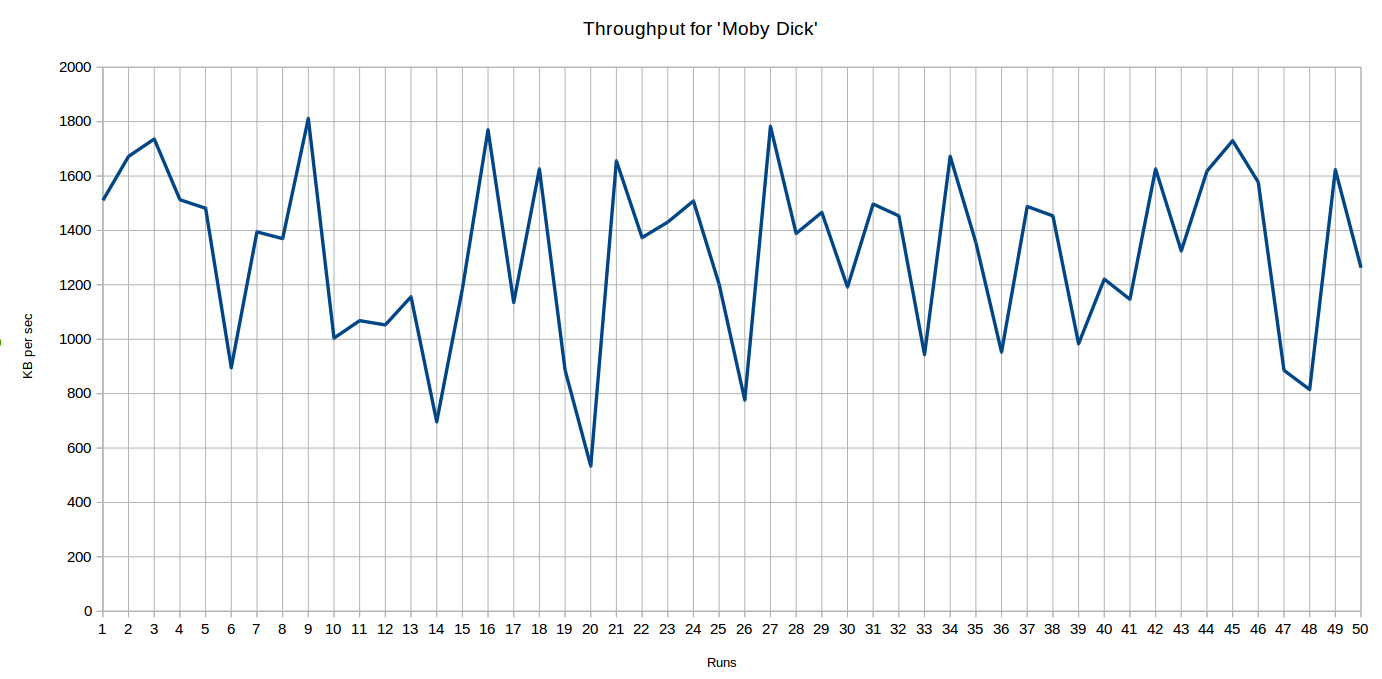
\includegraphics[height=8cm,keepaspectratio]{throughput.png}
  \caption{Graph of throughput. Variance $\approx 101381$, StDev $\approx 318$}
\end{figure}
\begin{figure}[!h]
  \centering
  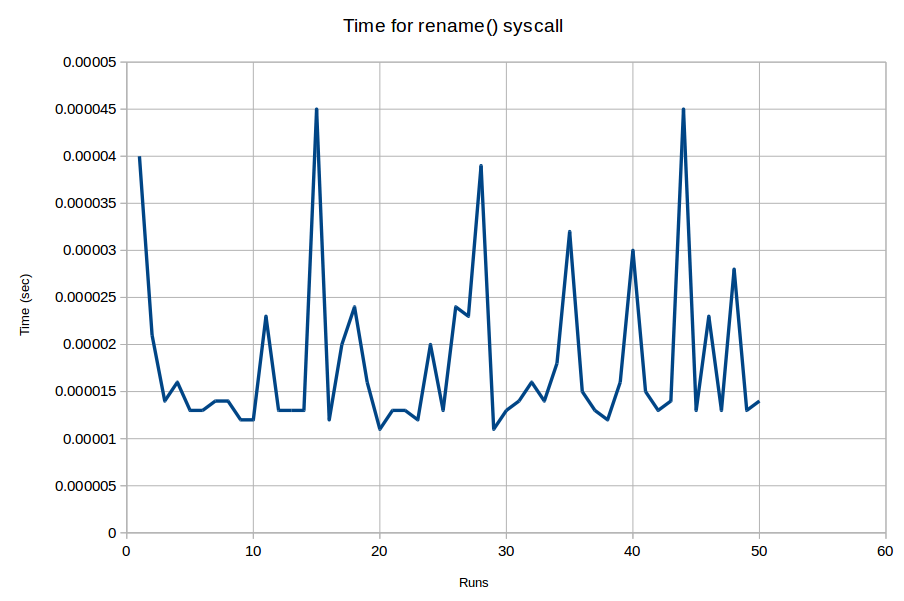
\includegraphics[height=8cm,keepaspectratio]{rename_times.png}
  \caption{Graph of times for rename(). I noticed no significant when
    files were larger instead of an empty .txt file. Variance $\approx 0.0000000000767$, StDev $\approx 0.00000876$}
\end{figure}
\newpage
\section*{Analysis}
All in all, these results suggest that while both sets of data indicate the operations are too fast to matter for small files, there is a non-significant amount of variance in both of them: The minimum times and throughputs were each smaller than the larger by a factor of 2. In particular for throughput, this suggests times to copy significantly large files might have much larger discrepancies in time. \\ \\
However, it is more than likely these variations could be restricted to small time measurements, and were caused by minor variations in resource allocation which are quite common in OSs. Overall, they are not likely to be of great concern, and are merely a side effect of the difficulty in making atomic, precise time measurements of programs.
\end{document}